% Apresentações em widescreen. Outros valores possíveis: 1610, 149, 54, 43 e 32.
% Por padrão, as apresentações são no formato 4:3 (sem o aspectratio).
\documentclass[aspectratio=43]{beamer}

\usetheme{Antibes}
\usecolortheme{default}
\usefonttheme[onlymath]{serif}			% para fontes matemáticas
% Enconte mais temas e cores em http://www.hartwork.org/beamer-theme-matrix/
% Veja também http://deic.uab.es/~iblanes/beamer_gallery/index.html
\bibliography{references}
% Customizações de Cores: fg significa cor do texto e bg é cor do fundo
\setbeamercolor{normal text}{fg=black}
\setbeamercolor{alerted text}{fg=red}
\setbeamercolor{author}{fg=black}
\setbeamercolor{institute}{fg=blue}
\setbeamercolor{date}{fg=black}
\setbeamercolor{frametitle}{fg=white}
\setbeamercolor{framesubtitle}{fg=brown}
\setbeamercolor{block title}{bg=blue, fg=white}		%Cor do título
\setbeamercolor{block body}{bg=gray, fg=darkgray}	%Cor do texto(bg= fundo; fg=texto)

% ---
% PACOTES
% ---
\usepackage[alf]{abntex2cite}		% Citações padrão ABNT
\usepackage[brazil]{babel}		% Idioma do documento
\usepackage{color}			% Controle das cores
\usepackage[T1]{fontenc}		% Selecao de codigos de fonte.
\usepackage{graphicx}			% Inclusão de gráficos
\usepackage[utf8]{inputenc}		% Codificacao do documento (conversão automática dos acentos)
\usepackage{gensymb}
\usepackage{txfonts}			% Fontes virtuais
% ---

% --- Informações do documento ---
\title{Apresentação da documentação do sistema Solus}
\author{Angelo Silva}
\institute{Instituto Federal de Educação, Ciência e Tecnologia de São Paulo Câmpus Boituva
	    \par
	    Curso de Análise e Desenvolvimento de sistemas}
\date{\today, v-1.0.0}
% ---

% ----------------- INÍCIO DO DOCUMENTO --------------------------------------
\begin{document}

\frame{\titlepage}

% ----------------- NOVO SLIDE --------------------------------
\begin{frame}{Sumário}
\tableofcontents
\end{frame}

\begin{frame}{Introdução}
\section{Introdução}

Na sociedade contemporânea, diversas preocupações quanto a captação de energia surgiram. Uma dessas preocupações é cada vez mais, buscar fontes renováveis de energia.
\end{frame}

\begin{frame}{Descrição geral do sistema}
\section{Descrição geral do sistema}
O projeto visa, através da análise estatística de dados meteorológicos, auxiliar o estudo de viabilidade acerca da instalação de painéis fotovoltaicos.

Para isso, serão coletados dados através de sensores conectados a um microcontrolador arduino. Inicialmente, prevemos captar informações de umidade do ar, temperatura e incidência de radiação solar.
\end{frame}

\begin{frame}{Requisitos do sistema}
\section{Requisitos do sistema}

\begin{figure}[H]
    \label{figure_diagrama_caso_uso}
    \centering
    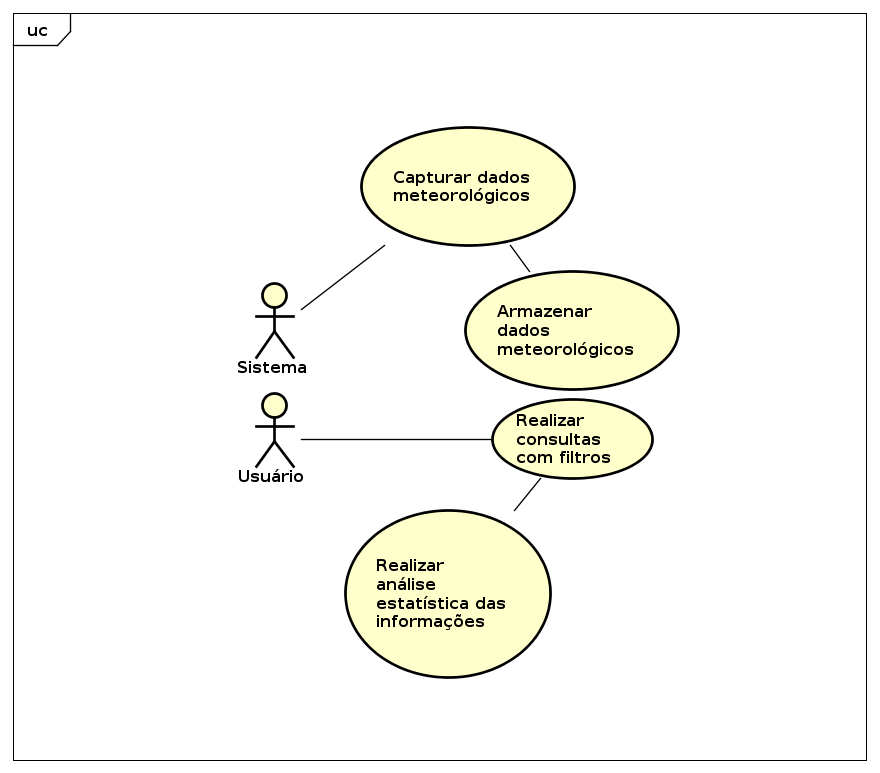
\includegraphics[scale=0.3]{caso_de_uso.png}
    \hfill
\end{figure}
\end{frame}

\begin{frame}{Requisitos não funcionais}
\section{Requisitos não funcionais}
\begin{itemize}
\item Segurança
\item Disponibilidade
\item Performance \ldots
\end{itemize}
\end{frame}

\begin{frame}{Regras de negócio}
\section{Regras de negócio}
A maior parte das regras de negócio de sistema fica centralizada nos filtros, eles são quem validam os dados do sistema, definindo regras para a captura de dados.

\begin{enumerate}
\item{Uma temperatura não pode se diferenciar em 25 $^{\circ}$C ou mais da média do último minuto}
\item{Uma temperatura não pode ser menor que \num{-100} $^{\circ}$C}
\item{Uma temperatura não pode ser maior que \num{+65} $^{\circ}$C}
\item{Uma temperatura não pode se diferenciar 5 $^{\circ}$C ou mais da anterior}
\end{enumerate}
\end{frame}

\begin{frame}{Estrutura de classes}
\section{Estrutura de classes}
    \begin{figure}[H]
        \label{figure_diagrama_classe}
        \centering
        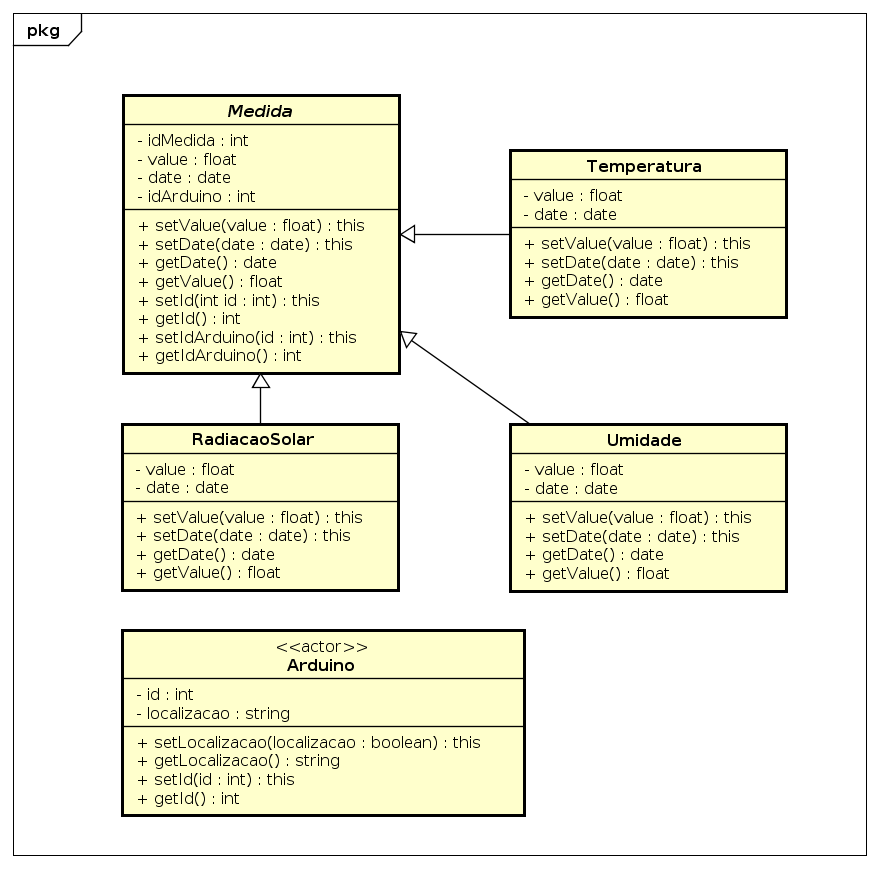
\includegraphics[scale=0.28]{classe.png}
        \hfill
    \end{figure}
\end{frame}

\begin{frame}{Estrutura de banco de dados}
\section{Estrutura de banco de dados}
    \begin{figure}[H]
        \label{figure_diagrama_banco}
        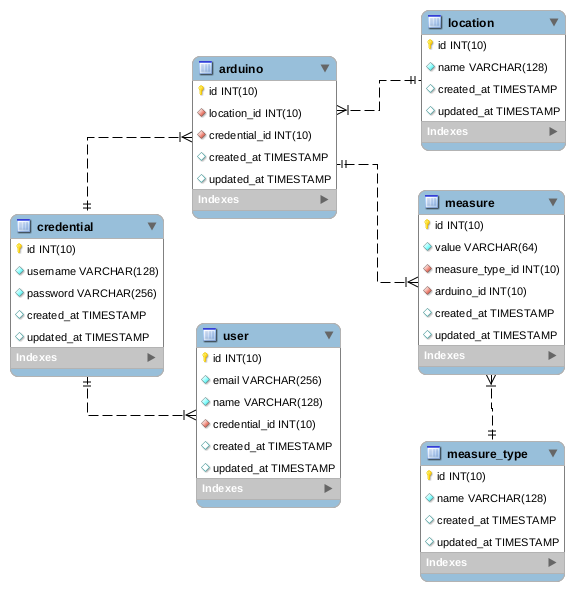
\includegraphics[scale=0.33]{scheme.png}
        \centering
        \hfill
    \end{figure}
\end{frame}

\begin{frame}{Diagrama de sequência}
\section{Diagrama de sequência}
    \begin{figure}[H]
        \label{figure_diagrama_sequencia}
        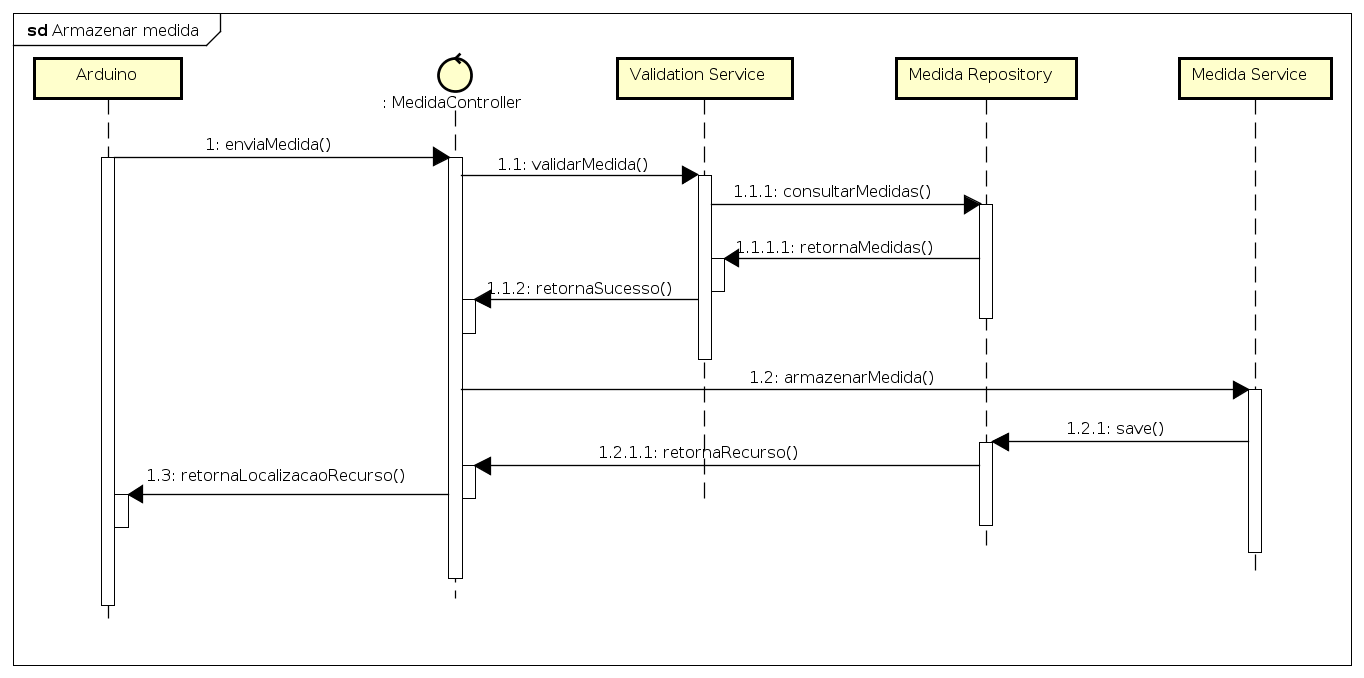
\includegraphics[scale=0.33]{sequencia.png}
        \centering
        \hfill
    \end{figure}
\end{frame}

\begin{frame}{Especificação das rotas da API}
\section{Especificação das rotas da API}
    \begin{table}[H]
        \centering
        \label{table_api_routes}
        \resizebox{\textwidth}{!}{
        \begin{tabular}{|l|l|l|}
        \hline
        \textbf{Método} & \textbf{Rota}        & \textbf{Descrição}                           \\ \hline
        GET             & /arduino             & Lista os arduinos                            \\ \hline
        GET             & /arduino/:id         & Retorna os dados de um arduino               \\ \hline
        POST            & /arduino             & Cadastra um novo arduino                     \\ \hline
        POST, PATCH     & /arduino/:id         & Atualiza os dados de um arduino              \\ \hline
        DELETE          & /arduino/:id         & Deleta um arduino e suas medidas capturadas  \\ \hline
        GET             & /arduino:id/measure  & Retorna as medidas capturadas por um arduino \\ \hline
        POST            & /arduino/:id/measure & Cadastra uma medida em um arduino            \\ \hline
        GET             & /measure/:id         & Retorna os dados de uma                \\ \hline
        POST            & /authenticate        & Retorna o Json Web Token de uma credencial   \\ \hline
        POST            & /location            & Cria uma nova localização                    \\ \hline
        GET             & /location/:id        & Retorna os dados de uma localização          \\ \hline
        POST, PATCH     & /location/:id        & Atualiza os dados de uma localização         \\ \hline
        DELETE          & /location/:id        & Deleta uma localização                       \\ \hline

        \end{tabular}}
    \end{table}
\end{frame}

% --- O comando \allowframebreaks ---
% Se o conteúdo não se encaixa em um quadro, a opção allowframebreaks instrui
% beamer para quebrá-lo automaticamente entre dois ou mais quadros,
% mantendo o frametitle do primeiro quadro (dado como argumento) e acrescentando
% um número romano ou algo parecido na continuação.no
% \begin{frame}[allowframebreaks]{Referências}
% \end{frame}

% ----------------- FIM DO DOCUMENTO -----------------------------------------
\end{document}
